\chapter{Forschungsergebnisse}

\section{Rangliste der Evaluationsverfahren}
In den folgenden beiden Tabellen \ref{tab:EI-EV-20} und \ref{tab:EI-EV-160} sind die Ergebnisse der Evaluationsverfahren für den zweiten Implementierungsabschnitt enthalten, welche nach Rang bzw. aufsteigend nach bester Algorithmus-Kombination geordnet sind. Der Rang ergibt sich dabei aus dem Mittelwert der normalisierten Werte der Metriken (Davies-Bouldin Index invertiert normalisiert). Die optimalen Werte für die verschiedenen Verfahren sind wie folgt:
\begin{itemize}
    \item Silhouette Score: 0,5 oder höher
    \item Caliński-Harabasz Index: höchster Wert aus allen Tests
    \item Davies-Bouldin Index: niedrigester Wert zwischen 0,3 und 0,7
\end{itemize}
Tabelle \ref{tab:EI-EV-20} legt nahe, dass UMAP das geeigneteste Dimensionsreduktionsverfahren ist, unabhängig vom Clustering-Algorithmus, wobei t-SNE und PCA mittelwertige Ergebnisse mit k-Means und schlechtere Ergebnisse mit HDBSCAN liefern.
Tabelle \ref{tab:EI-EV-160} zeigt, dass sich die Eignung nicht großartig ändert. So sind sowohl für kleine, als auch große Dateimengen beide Clustering-Algorithmen zusammen mit UMAP geeignet.

\setlength{\tabcolsep}{5.5pt}
\begin{table}[h]
\centering
\begin{tabular}{lcccc}
\hline
\textbf{Kombination} & \textbf{Silhouette} & \textbf{Calinski-Harabasz} & \textbf{Davies-Bouldin} & \textbf{Rang} \\
\hline
umap\_kmeans    & 0.763 & 3593.558 & 0.317 & 1 \\
umap\_hdbscan   & 0.728 & 3248.739 & 0.425 & 2 \\
tsne\_kmeans    & 0.640 & 173.360  & 0.273 & 3 \\
pca\_kmeans     & 0.609 & 168.268  & 0.444 & 4 \\
pca\_hdbscan    & 0.573 & 85.872   & 0.777 & 5 \\
tsne\_hdbscan   & 0.600 & 2.318    & 5.856 & 6 \\
\hline
\end{tabular}
\caption{Evaluationsergebnisse mit 40 Dateien.}
\label{tab:EI-EV-20}
\end{table}

\setlength{\tabcolsep}{5.5pt}
\begin{table}[h]
\centering
\begin{tabular}{lcccc}
\hline
\textbf{Kombination} & \textbf{Silhouette} & \textbf{Calinski-Harabasz} & \textbf{Davies-Bouldin} & \textbf{Rang} \\
\hline
umap\_kmeans    & 0.595 & 6554.361 & 0.390 & 1 \\
umap\_hdbscan   & 0.671 & 1398.606 & 0.608 & 2 \\
tsne\_kmeans    & 0.579 & 490.225  & 0.609 & 3 \\
pca\_kmeans     & 0.716 & 36.378   & 0.863 & 4 \\
pca\_hdbscan    & 0.408 & 201.754  & 0.780 & 5 \\
tsne\_hdbscan   & 0.421 & 267.712  & 0.814 & 6 \\
\hline
\end{tabular}
\caption{Evaluationsergebnisse mit 320 Dateien.}
\label{tab:EI-EV-160}
\end{table}


\section{Clustern unterschiedlicher Dateien in einem Diagramm}
\label{abs:C-u-D-i-e-D}
Folgende Abbildungen zeigen Clusterungen mit steigender Anzahl Dateien, die sich auf den zweiten Implementierungsabschnitt beziehen. Dabei trat das Problem auf, dass bei größeren Dateimengen die Wahrscheinlichkeit für gemischte Cluster, also mit unterschiedlichen Dateien in einem Cluster anstieg. In den Abbildungen \ref{abb:C-160-gC} und \ref{abb:C-160-gC-z} ist die Clusterung von 160 Point.java- (orangene Punkte) und 160 Circle.java-Dateien (blaue Punkte) und das beschriebene Problem zu sehen. Die genutzte Algorithmen-Kombination war UMAP mit HDBSCAN. Andere Kombinationen wie PCA mit k-Means ergaben deutlich andere Ergebnisse, jedoch stieg hier die Anzahl der gemischten Cluster ebenso an.

\begin{figure} %[hbtp]
	\centering
	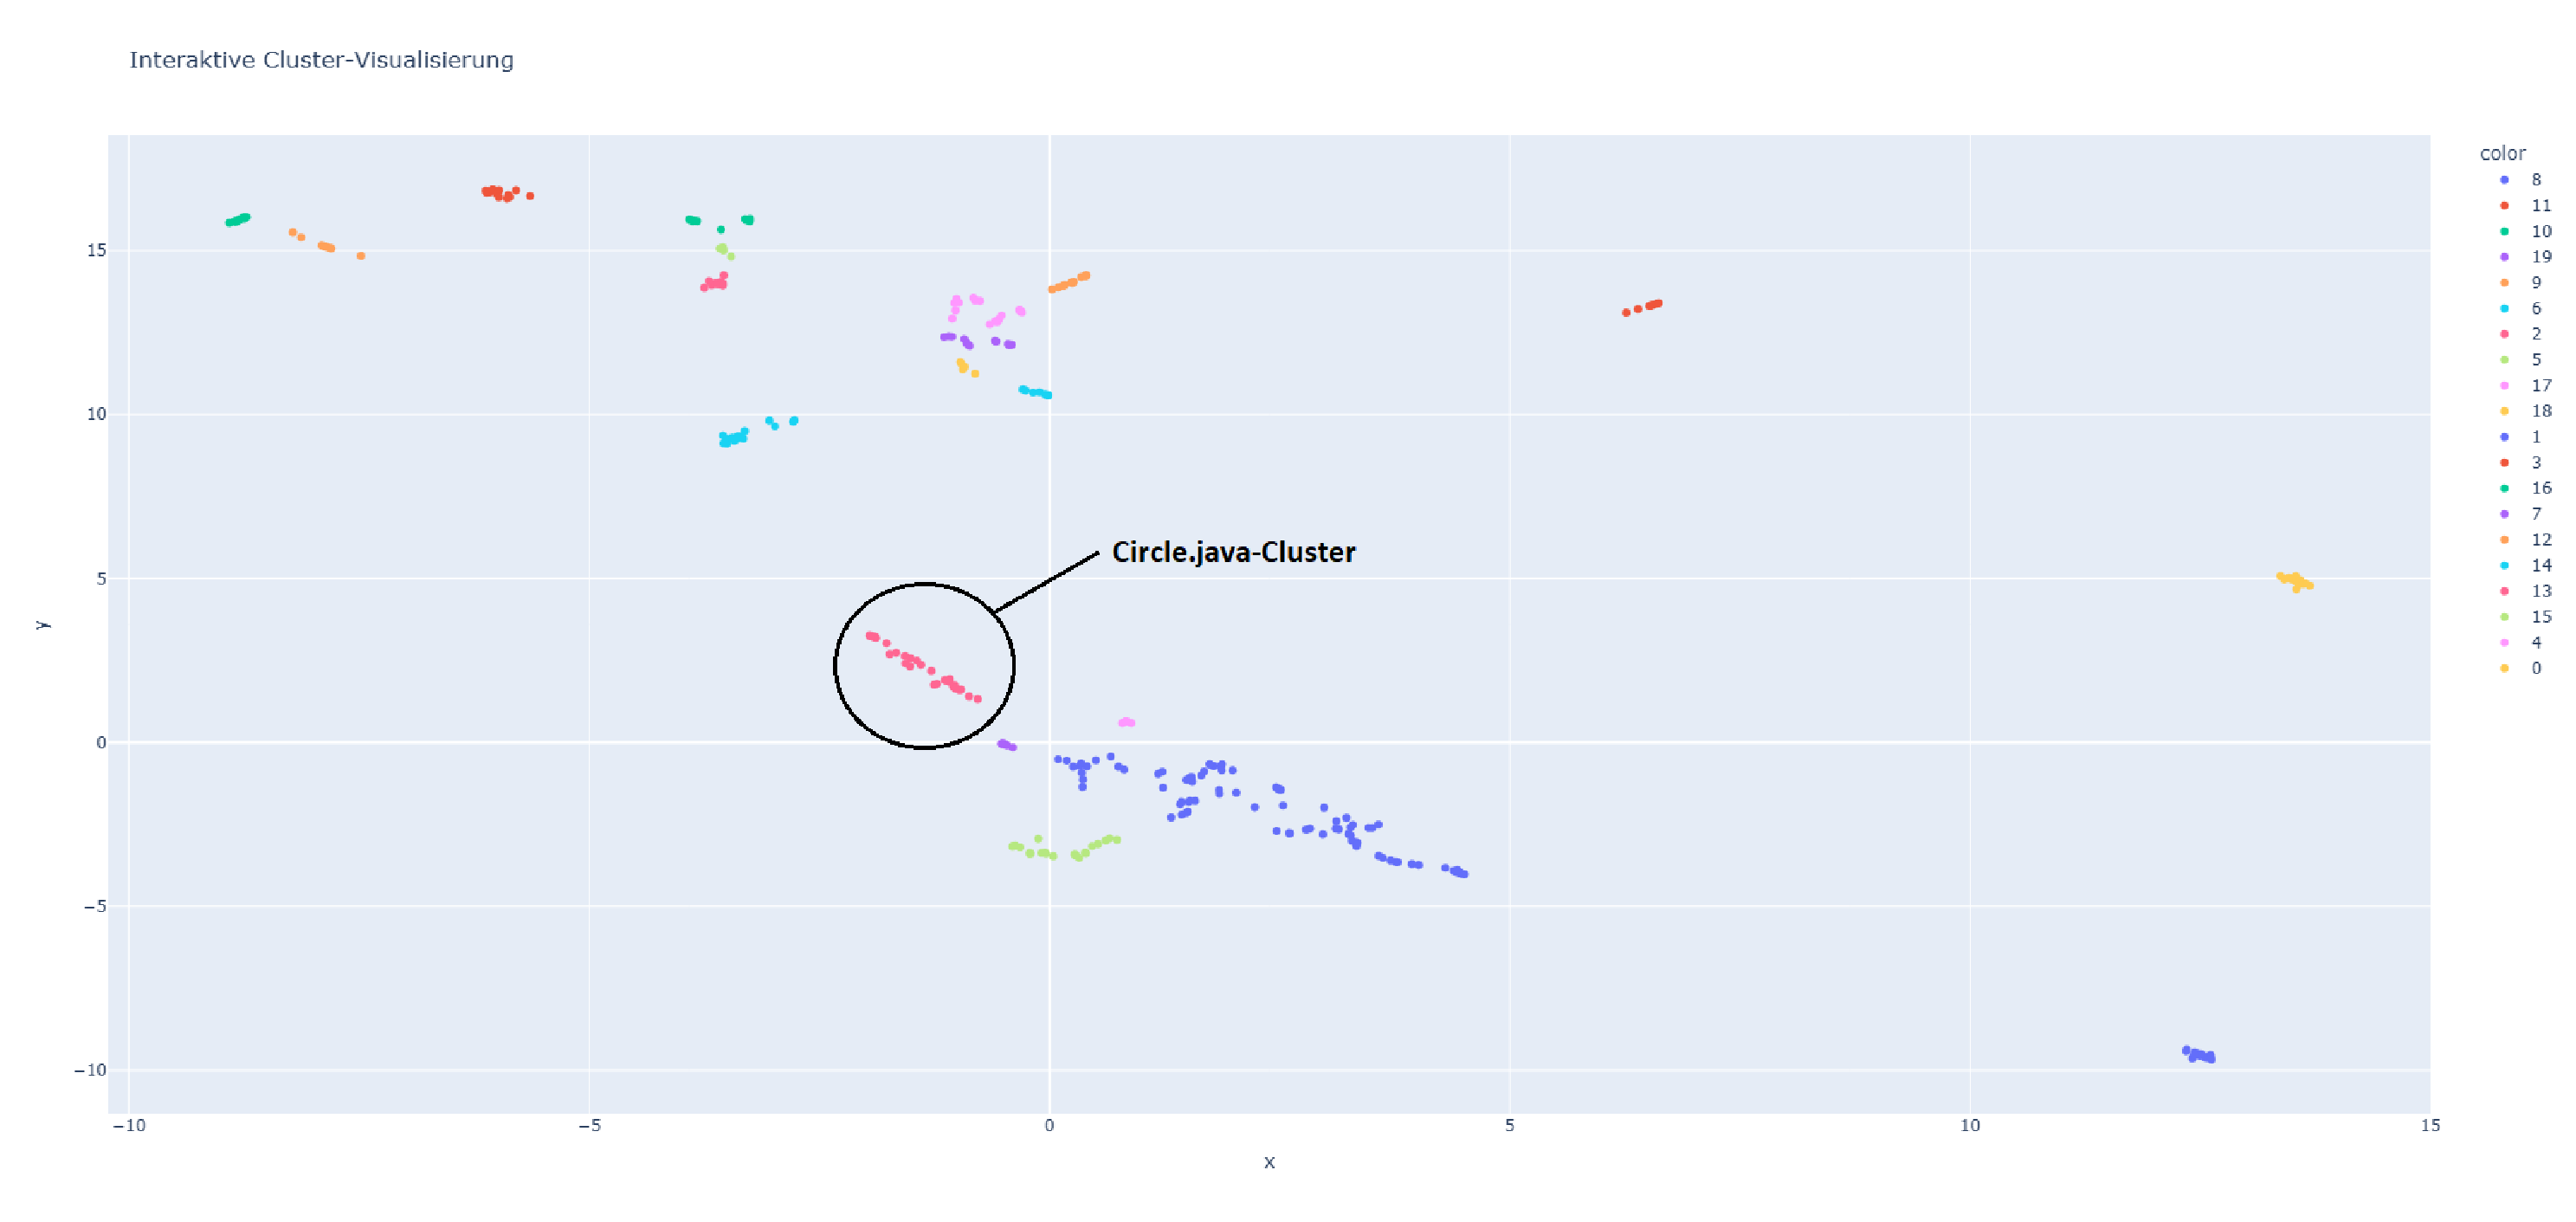
\includegraphics[width=1.0\textwidth]{images/Clusterung - 160 - gemischte Cluster.pdf}
	\caption{Clustering-Diagramm einer Clusterung von 320 Java-Dateien. Der eingekreiste Cluster ist ein Circle.java-Cluster.}
	\label{abb:C-160-gC}
\end{figure}

\begin{figure} %[hbtp]
	\centering
	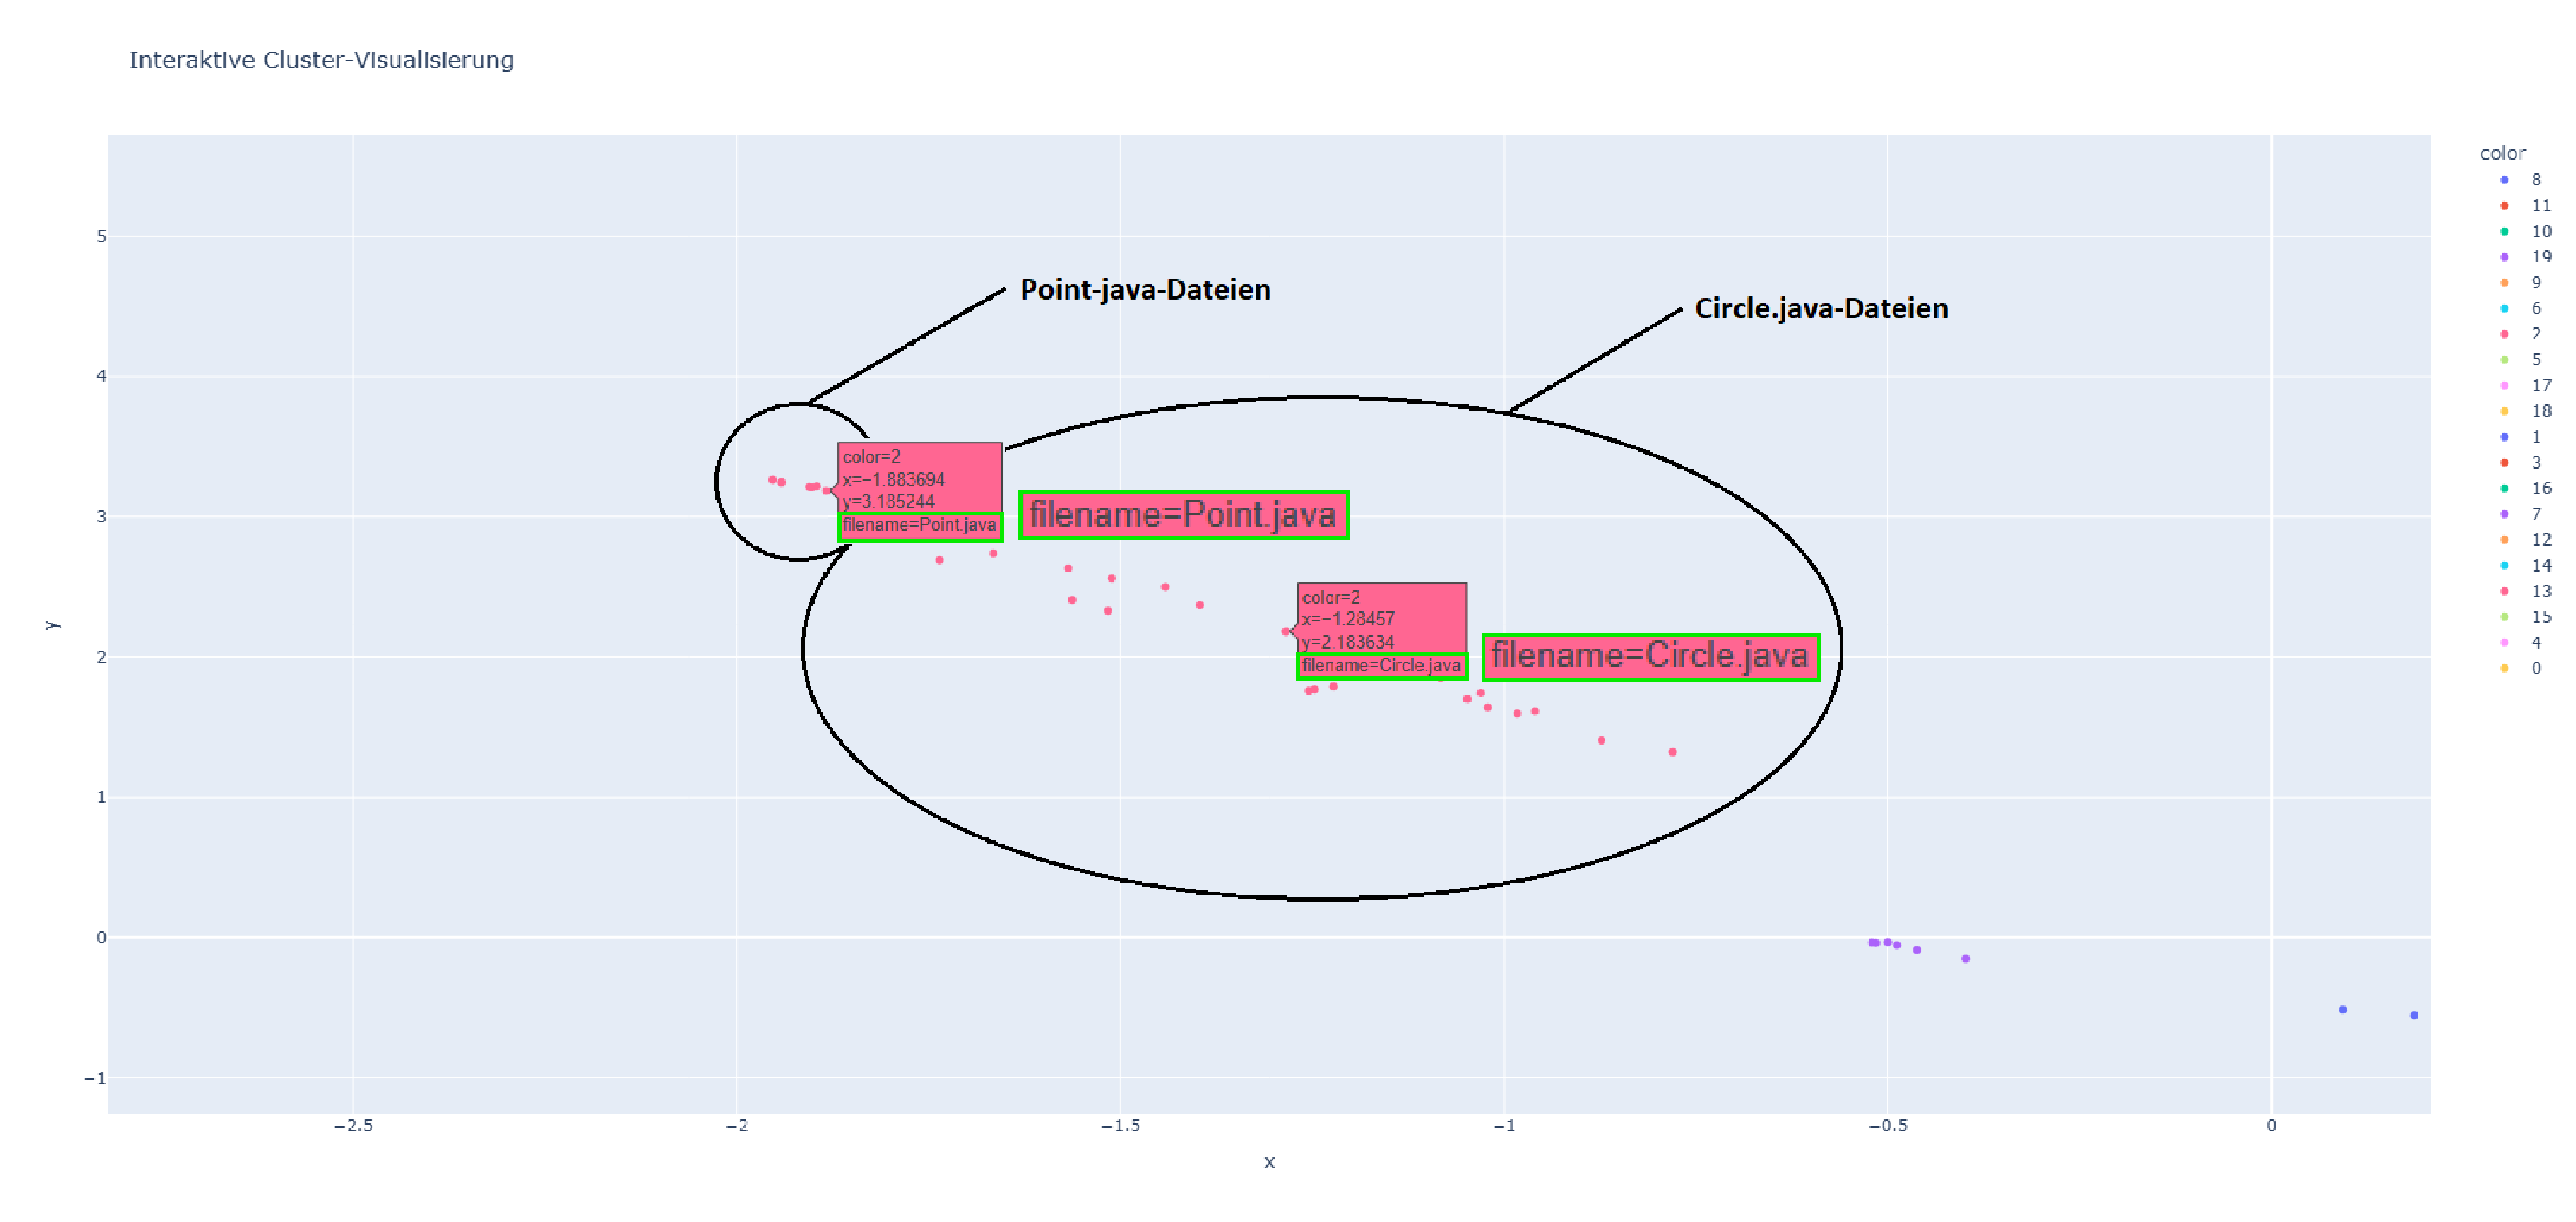
\includegraphics[width=1.0\textwidth]{images/Clusterung - 160 - gemischte Cluster - zoom.pdf}
	\caption{Vergrößerter Circle.java-Cluster aus Abbildung \ref{abb:C-160-gC}}
	\label{abb:C-160-gC-z}
\end{figure}